
\chapter{Dancing Links}
\label{dancing_links}

Dancing Links (DLX) is an algorithm invented by Donald Knuth to solve any exact cover problem.
It was first described in \cite{knuth00dancing} where he looks at the details of the algorithm and uses it to solve some practical problems.
Before we look at the DLX algorithm in more detail we need to explain what an exact cover problem is.
%The following section describes the exact cover problem in more detail.



\section{Exact cover}
\label{exact_cover}

Exact cover is a general type of problem which hcan be applied to a wide area of problems.
It can be used to solve problems like $N$ queens, polyomino tiling, Latin square puzzles, Sudoku, set packing and set partitioning.
More detailed information about how exact cover can be applied to $N$ queens, polyomino tiling, latin square and Sudoku can be found in Section \ref{queens_trans}, \ref{poly_trans}, \ref{latin_trans} and \ref{sudoku_trans} respectively.

To represent an exact cover problem we use a matrix in which each element is either zero or one (non-zero).
This type of matrix is called a boolean, binary, logical or \{0,1\}-matrix.
We use matrix in the rest of this report to mean a boolean matrix and non-zero to mean one since a boolean matrix can only have elements zero or one.
The idea is that each column in the matrix represents a specific constraint and each row is a way to fill some of the constraints.

For the general matrix
\begin{equation}
A =
\left[
\begin{array}{ccccc}
	a_{1,1} & a_{1,2} & a_{1,3} & \cdots & a_{1,n} \\
	a_{2,1} & a_{2,2} & a_{2,3} & \cdots & a_{2,n} \\
	a_{3,1} & a_{3,2} & a_{3,3} & \cdots & a_{3,n} \\
	\vdots  & \vdots  & \vdots  & \ddots & \vdots  \\
	a_{m,1} & a_{m,2} & a_{m,3} & \cdots & a_{m,n} \\
\end{array}
\right]
\label{eq:gen_cover_matrix}
\end{equation}
$a_{i,j}$ is an element in the matrix at row $i$, column $j$ where $a_{i,j} \in \{0,1\}$.
The number of rows is $m$ and the number of columns is $n$.

A subset of rows from a matrix is an exact cover iff (if and only if) each column has exactly one non-zero (one) element.
Let $R_A$ and $R_B$ be the set of rows in matrix $A$ and $B$ respectively.
When $R_B \subseteq R_A$ matrix $B$ forms the following matrix
\begin{equation}
	B =
	\left[
	\begin{array}{ccccc}
		b_{1,1} & b_{1,2} & b_{1,3} & \cdots & b_{1,n} \\
		b_{2,1} & b_{2,2} & b_{2,3} & \cdots & b_{2,n} \\
		b_{3,1} & b_{3,2} & b_{3,3} & \cdots & b_{3,n} \\
		\vdots  & \vdots  & \vdots  & \ddots & \vdots  \\
		b_{k,1} & b_{k,2} & b_{k,3} & \cdots & b_{k,n} \\
	\end{array}
	\right]
	\label{eq:cover_matrix}
\end{equation}
$B$ is a reduced matrix of $A$ where the number of rows $k \leq m$.
The number of columns in $A$ and $B$ is always the same.
The subset $R_B$ is an exact cover iff the following equation is satisfied
\[
	\sum_{i = 1}^{k} b_{i,j} = 1 \;\;\; \forall j \in \{ 1, 2, \ldots, n-1, n \}
\]

In practical applications we are usually given an initial matrix $A$ and tasked with finding all the subsets of rows which are exact covers.
For example the matrix
\begin{equation}
	\left[
	\begin{array}{cccc}
		1 & 0 & 0 & 0 \\
		0 & 1 & 1 & 0 \\
		1 & 0 & 0 & 1 \\
		0 & 0 & 1 & 1 \\
		0 & 1 & 0 & 0 \\
		0 & 0 & 1 & 0 \\
	\end{array}
	\right]
	\label{eq:cover_example}
\end{equation}
represents a specific exact cover problem.
In this matrix $\{ 2, 3 \}$ is one solution (exact cover) because the subset consisting of rows 2 and 3, and thus the reduced matrix
\[
\left[
\begin{array}{cccc}
	0 & 1 & 1 & 0 \\
	1 & 0 & 0 & 1 \\
\end{array}
\right]
\]
has exactly one non-zero element in each column.
By adopting a trial and error approach one can find that the full set of solutions for the matrix is $\{ \{1, 4, 5 \}, \{ 2, 3\}, \{ 3, 5, 6\} \}$.


\subsection{Generalized exact cover}

A generalized form of the exact cover problem is sometimes better suited to solve certain types of problems.
The generalized problem can be translated to an exact cover problem by adding additional rows, but translating in the opposite direction is not always possible.
The generalized cover problem divides the matrix into primary and secondary columns.
Each primary column in the solution must have exactly one non-zero element, like before.
However, each secondary column in a solution can have either zero or one non-zero element, instead of exactly one.

Let $C_P$ be the set of primary columns and $C_S$ the set of secondary columns in matrix $A$ and $B$.
The subset of rows $R_B$ is an exact cover iff the following two equations are satisfied
\[
	\sum_{i = 1}^{k} b_{i,j} = 1 \;\;\; \forall j \in C_P  \;\;\; \wedge \;\;\;  \sum_{i = 1}^{k} b_{i,j} \leq 1 \;\;\; \forall j \in C_S
\]


$N$ queens (see Section \ref{queens_trans}) is one type of problem the generalized cover problem can be applied to.
By creating a secondary column for each diagonal on the chess board will reduce the number of rows in the final matrix.
Given a smaller matrix the DLX algorithm will have to do less processing to find the solutions which results in better performance.



\section{Algorithm X}
\label{algox}

Exact cover is a type of problem known to be NP-complete.
To find all the solutions to an exact cover problem the most straight forward algorithm is to check all possible sets of rows.
Given a set we then check to see if there is exactly one non-zero element in each column.
However, as the size of the matrix increases we will experience a combinatorial explosion on the number of possible sets to test.
The exact number of sets is $2^{m}-1$ given a matrix with $m$ rows.
The eight queens problem (see Section \ref{queens_trans}) which has a matrix consisting of 63 rows, gives an immense 9~223~372~036~854~775~808 sets.
Given that only 92 of these are valid solutions this simple algorithm can hardly be recommended.

Another approach, which is presented in Knuth's paper, is the Algorithm X (for the lack of a better name).
This backtrack algorithm uses a more intelligent elimination method to ``wriggle'' its way through the matrix and find all the solutions.
Looking at matrix (\ref{eq:cover_example}) we can easily determine that row 1 and 3 never can be in the same set.
They are in conflict with each other because both of them have a non-zero element in the first column.
Since there must be exactly one non-zero element in each column we can rule out any sets with both row 1 and 3.

Algorithm X uses similar logic to recursively traverse a search tree by backtracking.
A modified version of Knuth's original algorithm is presented below.
Changes are made to improve the readability, logical consistency and to make it easier to compare with the Dancing Links algorithm.
The algorithm is initially called with the matrix $A$ and the column header list $H$.
$H$ is initialized with the numbers $1, 2, \ldots, n-1, n$, where $n$ is the number of columns in $A$.

\begin{algorithm}[H]
	\caption{Algorithm X recursive search procedure.}
	\label{algox_code}
	\begin{distribalgo}[1]
		\PROCEDURE{search($A, H$)}
			\IF{$H$ is empty}
				\STATE Print solution and return.  \COMMENT{Base case for the recursion}
			\ENDIF
			\STATE Choose a column $c$.
			\FOREACH{row $r$ such that $a_{r,c} = 1$}
				\STATE Add $r$ to partial solution.
				\STATE Save state of matrix $A$ and list $H$.
				\FOREACH{column $j$ such that $a_{r,j} = 1$}
					\FOREACH{row $i$ such that $a_{i,j} = 1$, \textbf{except} $i = r$}
						\STATE Delete row $i$ from matrix $A$.
					\ENDFOR
					\STATE Delete column $j$ from matrix $A$ and list $H$.
				\ENDFOR
				\STATE Delete row $r$ from matrix $A$.
				\STATE search($A,H$)
				\STATE Restore state of matrix $A$ and list $H$.
				\STATE Remove $r$ from the partial solution.
			\ENDFOR
		\ENDPROC
	\end{distribalgo}
\end{algorithm}

If $H$ is empty the partial solution is an exact cover and the algorithm returns.
Otherwise, the algorithm chooses a column $c$ and loops through each row $r$ in $c$ with a non-zero element.
Any conflict between row $r$ and the remaining rows are resolved on lines 7 to 11.
The algorithm then calls itself recursively with the reduced matrix and column list.
This continues until all the rows with non-zero elements in column $c$ have been tested, in which case all the branches in the search tree have been traversed.

Any rule for choosing column $c$ will produce all the solutions, but there are some rules that work better than others.
Knuth uses what he refers to as the $S$ heuristic, which is to always picking the column with the least amount of non-zero elements.
This approach has proved to work well in a large number of cases so it is a reasonable rule to make use of in practice.

Using matrix (\ref{eq:cover_example}) as an example, we wish to demonstrate how Algorithm X works.
The columns and rows have been numbered to make it easier to keep track of them when the matrix is modified.
\begin{equation}
	\label{eq:ces1}
	\begin{array}{r} 1\\ 2\\ 3\\ 4\\ 5\\ 6 \end{array}
	\stackrel{
		\begin{array}{cccc} 1 & 2 & 3 & 4 \end{array}
	}{
		\begin{bmatrix}
			1 & 0 & 0 & 0 \\
			0 & 1 & 1 & 0 \\
			1 & 0 & 0 & 1 \\
			0 & 0 & 1 & 1 \\
			0 & 1 & 0 & 0 \\
			0 & 0 & 1 & 0 \\
		\end{bmatrix}
	}
\end{equation}
We begin by choosing column 1.
Looking at this column we choose row 1 where there is a non-zero element.
Our partial solution is now $\{ 1 \}$.
Row 1 only has one conflicting row which is row 3, which has a conflict in column 1.
So we remove column 1, row 1 and row 3 which results in the following matrix
\begin{equation}
	\label{eq:ces2}
	\begin{array}{r} 2\\ 4\\ 5\\ 6 \end{array}
	\stackrel{
		\begin{array}{ccc} 2 & 3 & 4 \end{array}
	}{
		\begin{bmatrix}
			1 & 1 & 0 \\
			0 & 1 & 1 \\
			1 & 0 & 0 \\
			0 & 1 & 0 \\
		\end{bmatrix}
	}
\end{equation}
This time we choose column 2 and row 2 so the partial solution is $\{ 1, 2 \}$.
Row 2 conflicts with all the remaining rows (row 5 in column 2 and row 4 and 6 in column 3).
After all the conflicts have been resolved the matrix itself is empty, but not the column list $H$.
Because there are no non-zero elements left the recursive call will return immediately (the loop condition at line 5 is not satisfied) and matrix (\ref{eq:ces2}) is restored.
This time we choose row 5 giving the partial solution $\{ 1, 5 \}$.
Row 5 conflicts with row 2 in column 2 and by eliminating the conflicts we get the following matrix
\begin{equation}
	\label{eq:ces3}
	\begin{array}{r} 4\\ 6 \end{array}
	\stackrel{
		\begin{array}{ccc} 3 & 4 \end{array}
	}{
		\begin{bmatrix}
			1 & 1 \\
			1 & 0 \\
		\end{bmatrix}
	}
\end{equation}
We choose column 3 and row 4 which gives the partial solution $\{ 1, 5, 4 \}$.
After all the conflicts are resolved the matrix is completely empty along with the column header list.
This tells us that $\{ 1, 5, 4 \}$ is one solution to this problem.

By continuing in the same manner we eventually find all the solutions and the search tree in Figure \ref{fig:ex_tree} emerges.
Each node $i,j$, for row $i$ and column $j$, indicates the choices made and the rectangular nodes is where the solutions were found.
The search tree is a binary tree as a result of the small matrix used in this example so this is not something that can be generalized.
\begin{figure}[H]
	\centering 
	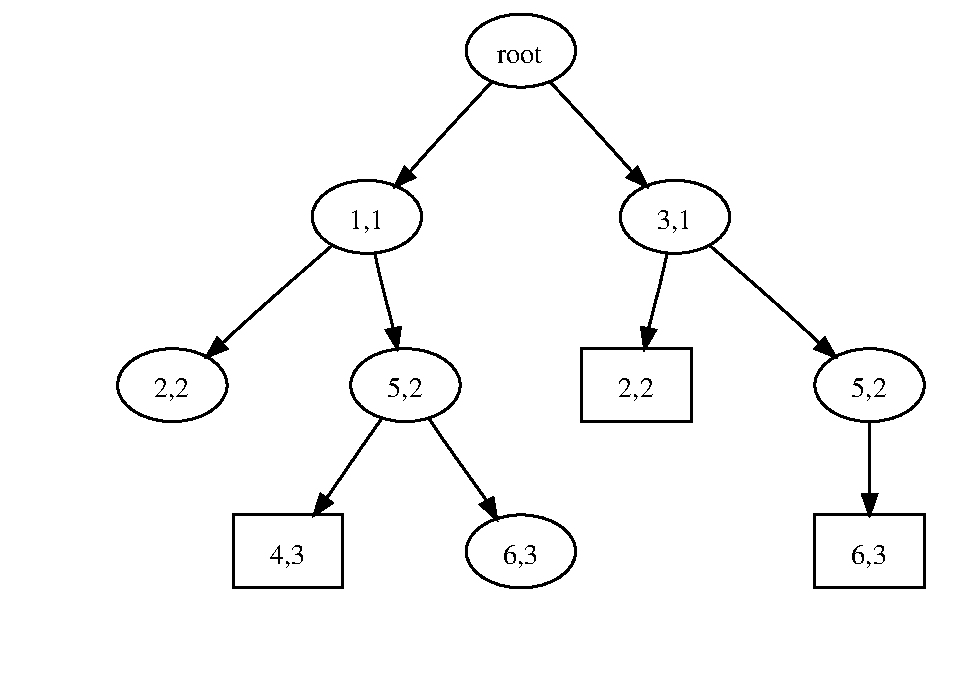
\includegraphics[width=0.85\textwidth]{search-tree-ex.pdf}
	\caption{Algorithm X search tree for the example matrix}
	\label{fig:ex_tree}
\end{figure}

One issue when trying to implement Algorithm X is that the state of the matrix needs to be saved and restored multiple times during the backtrack process.
Each time the algorithm returns the old state must be restored before another path can be explored.
Searching through the matrix to find the non-zero elements is also very time consuming if the matrix is stored as a two dimensional array.
To solve these problems Knuth introduced the Dancing Links algorithm.



\section{Dancing Links}
\label{dlx}

The Dancing Links (DLX) algorithm is based on Algorithm X, but it contains some significant modifications which makes it more suitable for practical applications.
DLX is based on a simple, yet powerful, technique which allows one to reverse any operation made to a doubly-linked list.
If $x$ represents an element in such a list then $x.left$ and $x.right$ points to the previous and next element, respectively.
To remove element $x$ from the list the following two operations are applied:
\begin{equation}
	\label{eq:remove}
	\begin{array}{rcl}
		x.right.left &\leftarrow& x.left \\
		x.left.right &\leftarrow& x.right \\
	\end{array}
\end{equation}

Applying these two operations to the linked list in Figure \ref{fig:linked} results in the list in Figure \ref{fig:linked_del}.
These operations modify the links pointing to element $x$ so that an iteration through the list will no longer traverse through this element, but instead skip right past it.
\begin{figure}[H]
	\centering 
	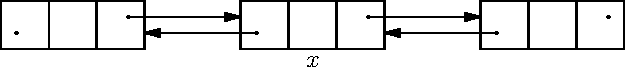
\includegraphics[width=0.8\textwidth]{doubly-linked-list.pdf}
	\caption{Doubly-linked list}
	\label{fig:linked}
\end{figure}
\begin{figure}[H]
	\centering 
	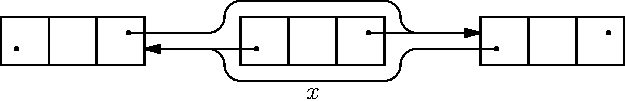
\includegraphics[width=0.8\textwidth]{doubly-linked-list-del.pdf}
	\caption{Doubly-linked list with element $x$ removed}
	\label{fig:linked_del}
\end{figure}

When programming one might be tempted to set $x.left$ and $x.right$ to a null value and delete the $x$ object or let the garbage collector do its thing.
However, smart as that might seem it would prevent one from applying a second set of operations.
In \cite{Hitotumatu79} Hitotumatu and Noshita introduced a pair of operations which allows one to insert an element back into the list in exactly the same place it was removed from.
The following two operations work as the inverse of the operations in (\ref{eq:remove}) by adding $x$ back to the list.
\begin{equation}
	\label{eq:add}
	\begin{array}{rcl}
		x.right.left &\leftarrow& x \\
		x.left.right &\leftarrow& x \\
	\end{array}
\end{equation}

Knuth makes use of the operations in (\ref{eq:remove}) and (\ref{eq:add}) to maintain the state information for the matrix.
The $x$ element is preserved so that the algorithm can reverse the remove operations, which is used to reduce the matrix.


\subsection{Data structure}
\label{dlx_struct}

DLX stores the matrix as a collection of several circular doubly-linked lists where each non-zero value in the matrix is an element in the lists.
Using this sparse matrix representation saves a lot of memory because the number of zero elements usually outnumber the non-zero elements.
This advantage will normally grow when the size of the matrix increases.
As an example the $N$ queens problem for $N=10$ has 396 non-zero elements, but they only account for 7.33\% of the total number of elements.

Each row and column in the matrix is represented by a separate list.
In addition the set of column headers is also stored in a list.
Each element $x$ in the linked lists have six attributes: $x.left$, $x.right$, $x.up$, $x.down$, $x.column$ and $x.row$.
The $x.row$ attribute is an addition to Knuth's original algorithm to enable detection of the row number.
The first four attributes contains a pointer to an element in the respective list.
$x.left$ and $x.right$ belongs to the row list and $x.up$ and $x.down$ belongs to the column list.
$x.column$ is a pointer to the column header and $x.row$ is a non-negative integer storing the row number of the element.
The column headers $c$ has the additional $c.name$ (column name/number) and $c.size$ (number of elements in column) attributes.
There is also a special column header element $h$ which acts as a root element.

Figure \ref{fig:matrix_links} shows shows how the matrix in (\ref{eq:cover_example}) can be represented using this data structure.
To avoid clutter the $x.column$ links pointing to the column headers is not displayed.
\begin{figure}[htbp]
	\centering
	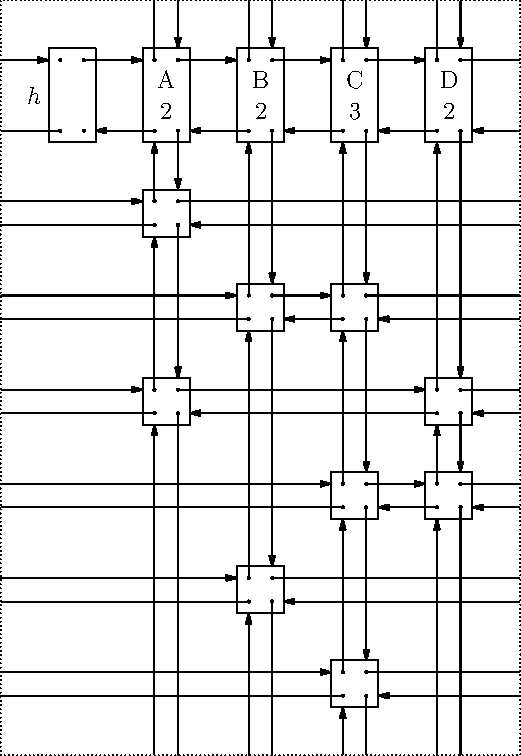
\includegraphics[width=0.8\textwidth]{matrix-links.pdf}
	\caption{Sparse boolean matrix circular quad-linked list representation of the example matrix}
	\label{fig:matrix_links}
\end{figure}


\subsection{Algorithm}

The DLX algorithm is very similar in nature to Algorithm X and in essence the two algorithms work exactly in the same way.
Given the example matrix (\ref{eq:cover_example}) the DLX algorithm will follow the same path as shown in Figure \ref{fig:ex_tree}.
The difference is that DLX uses a specialized data structure, and the operations in (\ref{eq:remove}) and (\ref{eq:add}) to save and restore the state of the matrix.
Comparing the pseudo code for the DLX algorithm below with Algorithm X reveals that they are very similar.
The algorithm is initially called with $k = 0$ (recursion level 0) and $h$ is initialized with the contents of the matrix.
See Section \ref{matrix_construction} for details on how the contents of $h$ is initialized.
Printing a solution using the $x.row$ attribute is done by printing $O_{i}.row$ for $i = \{1, 2, \ldots, k\}$.
\begin{algorithm}[H]
	\caption{Dancing Links recursive search.}
	\label{dlx_search}
	\begin{distribalgo}[1]
		\PROCEDURE{search($k$)}
			\IF{$h.right = h$}
				\STATE Print solution and return.  \COMMENT{Base case for the recursion}
			\ENDIF
			\STATE $c \leftarrow$ choose\_column()
			\STATE cover($c$)
			\FOREACH{$r \leftarrow c.down, c.down.down, \ldots,$ \textbf{while} $r \neq c$}
				\STATE $O_k \leftarrow r$  \COMMENT{Add $r$ to partial solution}
				\FOREACH{$j \leftarrow r.right, r.right.right, \ldots,$ \textbf{while} $j \neq r$}
					\STATE cover($j.column$)
				\ENDFOR
				\STATE search($k + 1$)
				\FOREACH{$j \leftarrow r.left, r.left.left, \ldots,$ \textbf{while} $j \neq r$}
					\STATE uncover($j.column$)
				\ENDFOR
			\ENDFOR
			\STATE uncover($c$)
		\ENDPROC
	\end{distribalgo}
\end{algorithm}

Column selection is done using the $S$ heuristic, which picks the column with the lowest value for $c.size$, as described in Knuth's paper.
The algorithm simply steps through each column header looking for the lowest size.
\begin{algorithm}[H]
	\caption{Column selection using the $S$ heuristic.}
	\label{dlx_column}
	\begin{distribalgo}[1]
		\FUNCTION{choose\_column()}
			\STATE $s \leftarrow \infty$
			\FOREACH{$j \leftarrow h.right, h.right.right, \ldots,$ \textbf{while} $j \neq h$}
				\IF{$j.size < s$}
					\STATE $c \leftarrow j$
					\STATE $s \leftarrow j.size$
				\ENDIF
			\ENDFOR
			\RETURN{column $c$}
		\ENDFUNC
	\end{distribalgo}
\end{algorithm}

The cover($c$) and uncover($c$) algorithms are the main differences compared to Algorithm X.
The purpose of cover($c$) is to remove column $c$ from the column header list and to resolve any conflicts in the column.
It uses the operations in (\ref{eq:remove}) to remove the conflicting elements from the column lists.
The cover algorithm also increments the value of $updates$ which is used to measure how many operations the search algorithm requires to complete.
One update equals four link changes or one application of both (\ref{eq:remove}) and (\ref{eq:add}).
\begin{algorithm}[H]
	\caption{Cover column $c$.}
	\label{dlx_cover}
	\begin{distribalgo}[1]
		\PROCEDURE{cover($c$)}
			\STATE $c.right.left \leftarrow c.left$
			\STATE $c.left.right \leftarrow c.right$
			\FOREACH{$i \leftarrow c.down, c.down.down, \ldots,$ \textbf{while} $i \neq c$}
				\FOREACH{$j \leftarrow i.right, i.right.right, \ldots,$ \textbf{while} $j \neq i$}
					\STATE $j.down.up \leftarrow j.up$
					\STATE $j.up.down \leftarrow j.down$
					\STATE $j.column.size \leftarrow j.column.size - 1$
					\STATE $updates \leftarrow updates + 1$
				\ENDFOR
			\ENDFOR
		\ENDPROC
	\end{distribalgo}
\end{algorithm}

The uncover($c$) algorithm restores the state of the matrix using the operations in (\ref{eq:add}).
Notice that this algorithm walks up and left in the lists while cover($c$) walks down and right.
This ensures that all the elements are put back in the reverse order in which they were removed.
\begin{algorithm}[H]
	\caption{Uncover column $c$.}
	\label{dlx_uncover}
	\begin{distribalgo}[1]
		\PROCEDURE{uncover($c$)}
			\FOREACH{$i \leftarrow c.up, c.up.up \ldots,$ \textbf{while} $i \neq c$}
				\FOREACH{$j \leftarrow i.left, i.left.left, \ldots,$ \textbf{while} $j \neq i$}
					\STATE $j.column.size \leftarrow j.column.size + 1$
					\STATE $j.down.up \leftarrow j$
					\STATE $j.up.down \leftarrow j$
				\ENDFOR
			\ENDFOR
			\STATE $c.right.left \leftarrow c$
			\STATE $c.left.right \leftarrow c$
		\ENDPROC
	\end{distribalgo}
\end{algorithm}



\section{Parallel Dancing Links}

To be able to solve more complex exact cover problems the solution process must be distributed to a larger number of computers.
To accomplish this we must first break the problem into smaller pieces.
In \cite{maus-prp} Maus and Aas investigates recursive procedures as the unit for parallelizing.
They introduce some techniques on how to split the recursion tree which can be directly applied to the search tree in DLX.
The main idea is that the algorithm is first run in a breath-first mode so that the search tree is explored one level at a time.
When a certain number of nodes has been discovered they are distributed to a set computers and solved in parallel.

The search procedure of DLX is a backtrack algorithm which explores the search tree depth-first.
Making this a breath-first algorithm can be achieved by not allowing it to proceed deeper than a certain level in the search tree.
When the given level is reached the partial solution is printed.
It can then be used to initialize a separate process running DLX on a different computer (or another processor on the same computer).
As long as the predefined depth $d$ is not too deep or shallow the partial solutions can be used to efficiently solve the exact cover problem in a distributed manner.
If $d$ is too deep (high) the algorithm will find all solutions before the splitting happens, and if it is too shallow (low) the number of partial solutions might be too low to be of any use.
\begin{algorithm}[H]
	\caption{Dancing Links parallel recursive splitter.}
	\label{dlx_dsearch}
	\begin{distribalgo}[1]
		\PROCEDURE{psearch($k, d$)}
			\IF{$h.right = h$}
				\STATE Print solution and return.  \COMMENT{Base case for the recursion}
			\ENDIF
			\STATE $c \leftarrow$ choose\_column()
			\STATE cover($c$)
			\FOREACH{$r \leftarrow c.down, c.down.down, \ldots,$ \textbf{while} $r \neq c$}
				\STATE $O_k \leftarrow r$  \COMMENT{Add $r$ to partial solution}
				\FOREACH{$j \leftarrow r.right, r.right.right, \ldots,$ \textbf{while} $j \neq r$}
					\STATE cover($j.column$)
				\ENDFOR
				\IF{$k = d$ and $h.right \neq h$}
					\STATE Print partial solution.
				\ELSE
					\STATE psearch($k + 1$)
				\ENDIF
				\FOREACH{$j \leftarrow r.left, r.left.left, \ldots,$ \textbf{while} $j \neq r$}
					\STATE uncover($j.column$)
				\ENDFOR
			\ENDFOR
			\STATE uncover($c$)
		\ENDPROC
	\end{distribalgo}
\end{algorithm}

Each partial solution can then be used as initialization vectors for the modified search procedure search\_init($O$) in Algorithm \ref{algo:dlx_isearch}.
$O$ is the initialization vector and $p$ is the length of the vector (number of rows in the partial solution).
The initialization vectors and the matrix can be distributed and the modified search procedure can be run in parallel on each computer.
If required each computer can do further splitting locally to take advantage of multiple processors.
\begin{algorithm}[H]
	\caption{Dancing Links search initialization.}
	\label{algo:dlx_isearch}
	\begin{distribalgo}[1]
		\PROCEDURE{search\_init($O$)}
			\FOR{$k \leftarrow 0$ to $p-1$}
				\STATE $c \leftarrow$ choose\_column()
				\STATE cover($c$)
				\STATE $r \leftarrow O_k$
				\FOREACH{$j \leftarrow r.right, r.right.right, \ldots,$ \textbf{while} $j \neq r$}
					\STATE cover($j.column$)
				\ENDFOR
			\ENDFOR
			\STATE search($p$)  \COMMENT{Do actual search}
		\ENDPROC
	\end{distribalgo}
\end{algorithm}

This approach does not guarantee that each initialization vector provides a similar amount of work.
Unfortunately there is straight forward method to estimate the complexity of the subtree given by a specific initialization vector.
In \cite{knuth75backtracking} Knuth uses a Monte Carlo approach to estimate the running time of backtrack algorithms.
By doing random walks in the subtree he is able to estimate the cost of backtracking.
It would be worth investigating this approach in more detail if DECS was to be extended.